
\chapter{Results}

\subsection*{\textit{Roller Painting} Navigation Strategy}

We summarize in figure~\ref{fig:peinture_au_rouleau-kappa_vs_world} the evolution of the Cohen score as a function of the density of the world for each value of $d$.
We also summarize in figure~\ref{fig:peinture_au_rouleau-time_vs_world} the evolution of the inspection time according to the density of the world for each value of $d$.

\begin{figure}[h!]
	\centering
	\begin{subfigure}[t]{0.9\linewidth}
		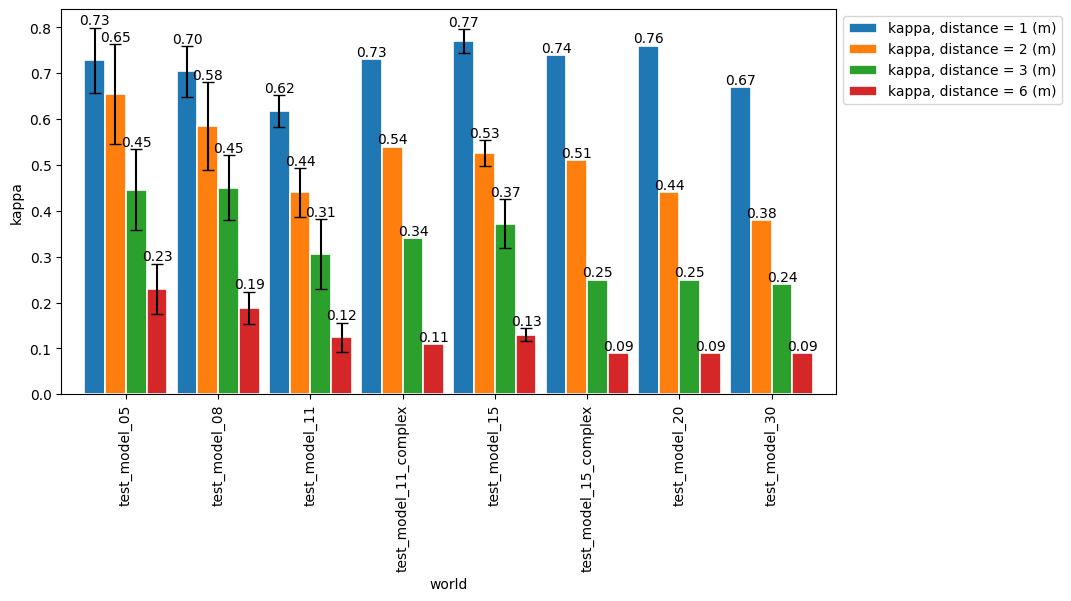
\includegraphics[width=\linewidth]{graphics/peinture_au_rouleau-kappa_vs_world_for_each_d.png}
		\caption{$\kappa$ according to the density of the world.}
		\label{fig:peinture_au_rouleau-kappa_vs_world}
	\end{subfigure}
	\hfill
	\begin{subfigure}[t]{0.9\linewidth}
			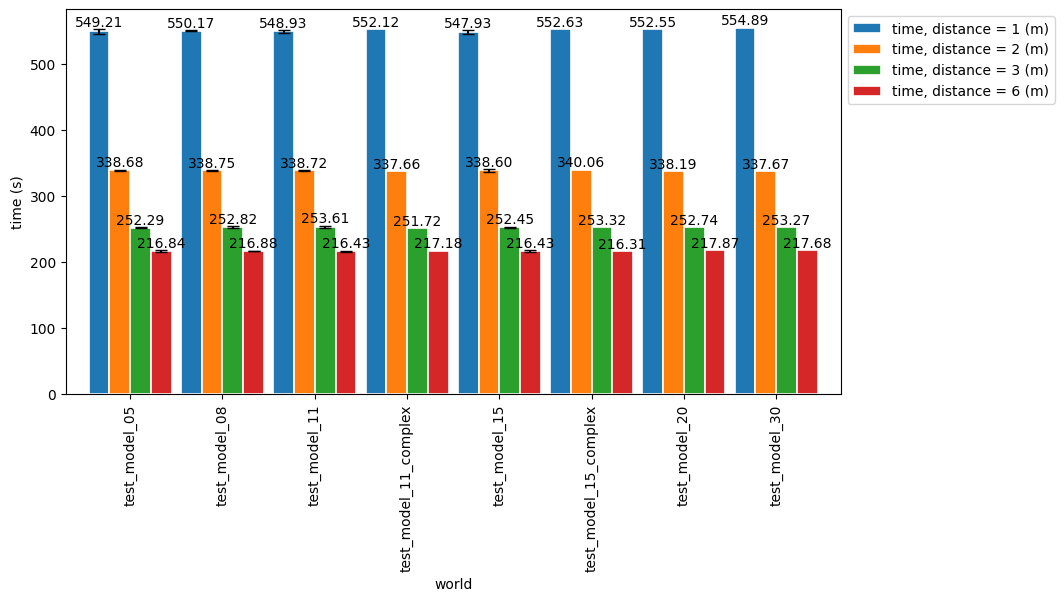
\includegraphics[width=\linewidth]{graphics/peinture_au_rouleau-time_vs_world_for_each_d.png}
			\caption{Runtime based on world density.}
			\label{fig:peinture_au_rouleau-time_vs_world}
	\end{subfigure}
	\caption{Evolution of Cohen's $\kappa$ and the execution time of the \textit{Roller Painting} algorithm as a function of the density of the world and the distance between the robots.}
	\label{fig:peinture_au_rouleau-world}
\end{figure}

First, we can observe that the Cohen score generally decreases with the number of corrosion zones.
There are exceptions, notably for the map composed of 15 corrosion zones, where the Cohen score is higher than for the maps composed of 5, 8 and 11 corrosion zones.
This is explained by the fact that in the maps composed of 5, 8 and 11 corrosion zones, we have introduced corrosion zones with elongated shapes unlike the map composed of 15 corrosion zones where the corrosion zones are all circles .
Indeed, elongated corrosion zones have a greater probability of causing phantom zones to appear, illustrated in figure~\ref{fig:ghost_zone}, than circular corrosion zones.
These phantom zones are areas free of corrosion which are detected by the crawlers.
These are therefore false positives which reduce the Cohen score.
These phantom zones are also more likely to appear when the density of the world is high and therefore the corrosion zones are closer to each other, or when the distance $d$ between the two crawlers is high.
This is what we can observe in figure~\ref{fig:peinture_au_rouleau-kappa_vs_distance} where the Cohen score decreases when the distance $d$ between the two crawlers increases.
We observe that there seems to be a linear relationship between the Cohen score and the distance $d$ between the two crawlers.

\begin{figure}[h!]
	\begin{subfigure}[t]{0.49\linewidth}
		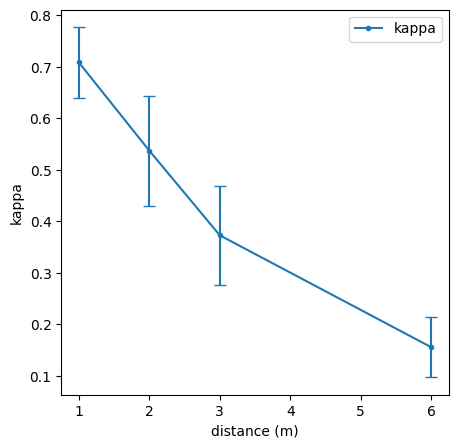
\includegraphics[width=\linewidth]{graphics/peinture_au_rouleau-kappa_vs_distance.png}
		\caption{$\kappa$ depending on the distance between the two crawlers.}
		\label{fig:peinture_au_rouleau-kappa_vs_distance}
	\end{subfigure}
	\hfill
	\begin{subfigure}[t]{0.49\linewidth}
			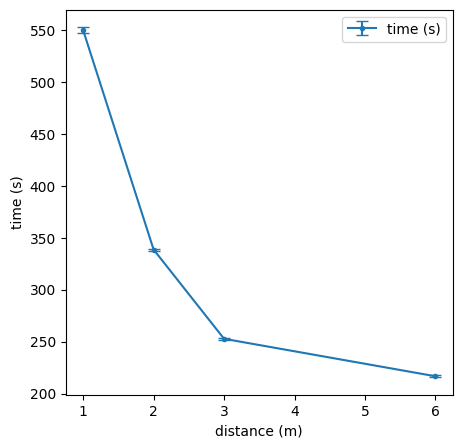
\includegraphics[width=\linewidth]{graphics/peinture_au_rouleau-time_vs_distance.png}
			\caption{Runtime depending on the distance between the two crawlers.}
			\label{fig:peinture_au_rouleau-time_vs_distance}
	\end{subfigure}
	\caption{Evolution of Cohen's $\kappa$ and the execution time of the \textit{Roller Painting} algorithm as a function of the distance between the two crawlers.}
	\label{fig:peinture_au_rouleau-distance}
\end{figure}

\begin{figure}[h!]
	\centering
	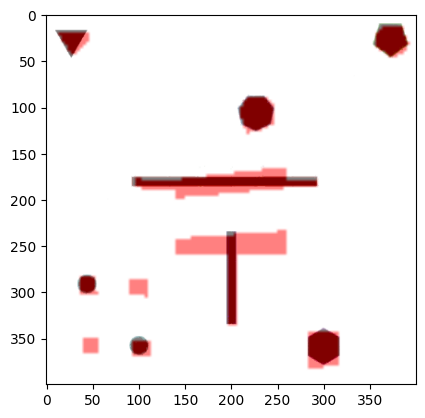
\includegraphics[width=0.5\linewidth]{graphics/output.png}
	\caption{Example of a phantom zone located at the bottom left of the map.}
	\label{fig:ghost_zone}
\end{figure}

Then, we observe that the execution time of the \textit{Roller Painting} algorithm is constant for each value of the number of corrosion zones.
This was expected because the algorithm in question is an \textit{a priori} algorithm and therefore does not depend on the number of corrosion zones.
On the other hand, the execution time depends on the distance $d$ between the two crawlers.
As we can see in figure~\ref{fig:peinture_au_rouleau-time_vs_distance}, the execution time increases when the distance $d$ between the two crawlers decreases.
This is because the greater the distance $d$, the fewer moves the crawlers have to make to cover the map.
There does not seem to be a linear relationship between the execution time and the distance $d$ between the two crawlers.
However, we would have expected that there would be a linear relationship between the execution time and the distance $d$ between the two crawlers.
It would be interesting to check if there was no bias introduced during the implementation of the algorithm.

We have also introduced two maps with more complex shapes than the base maps.
These are visible in the appendix~\ref{annexe:cartes}, in figures~\ref{fig:test_model_11_complex_1} and~\ref{fig:test_model_15_complex_1}.
Unfortunately, we could not, for the sake of time, vary the position of the corrosion zones, as we did with the low density maps.
However, there seems to be no significant difference between complex shaped maps and simple shaped maps.
For example, for the maps with 15 forms of corrosion and the map with 15 complex forms of corrosion, the Cohen score only varies by 0.02 on average for a distance $d = 1$ and by 0.04 on average for a distance $d = 6$.

In the rest of this report, we will consider a distance $d = 3$ meters between the two crawlers for the \textit{Roller Painting} algorithm.

\subsection*{\textit{Nordic Skiing} Navigation Strategy}

We are now going to analyze the results obtained for the \textit{Nordic Skiing} algorithm.
As for the \textit{Roller Painting} algorithm, we varied the density of the world and the distance $d$ between the two crawlers, but also the stride $s$ used between the two crawlers.
The figure~\ref{fig:ski_nordique-world_d} presents the evolution of the Cohen score and the execution time of the algorithm \textit{Nordic Skiing} as a function of the density of the world for different values of the distance $d$ between the two crawlers and a stride $s = 3$ meters.

\begin{figure}[h!]
	\centering
	\begin{subfigure}[t]{0.9\linewidth}
		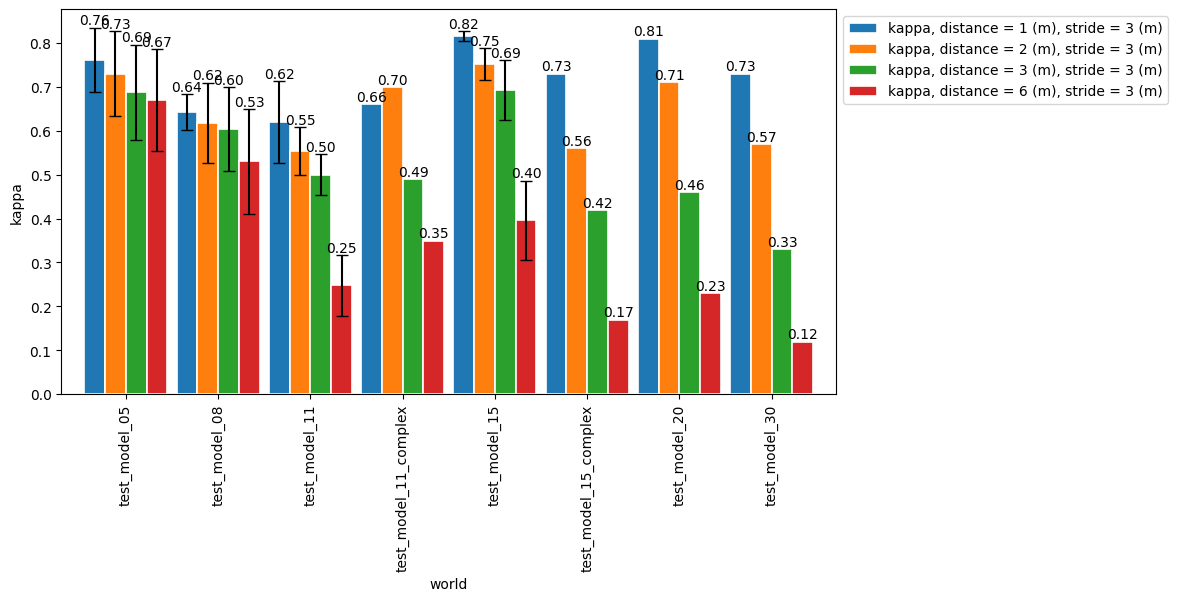
\includegraphics[width=\linewidth]{graphics/ski_nordique-kappa_vs_world_for_each_d.png}
		\caption{$\kappa$ according to the density of the world.}
		\label{fig:ski_nordique-kappa_vs_world_d}
	\end{subfigure}
	\hfill
	\begin{subfigure}[t]{0.9\linewidth}
		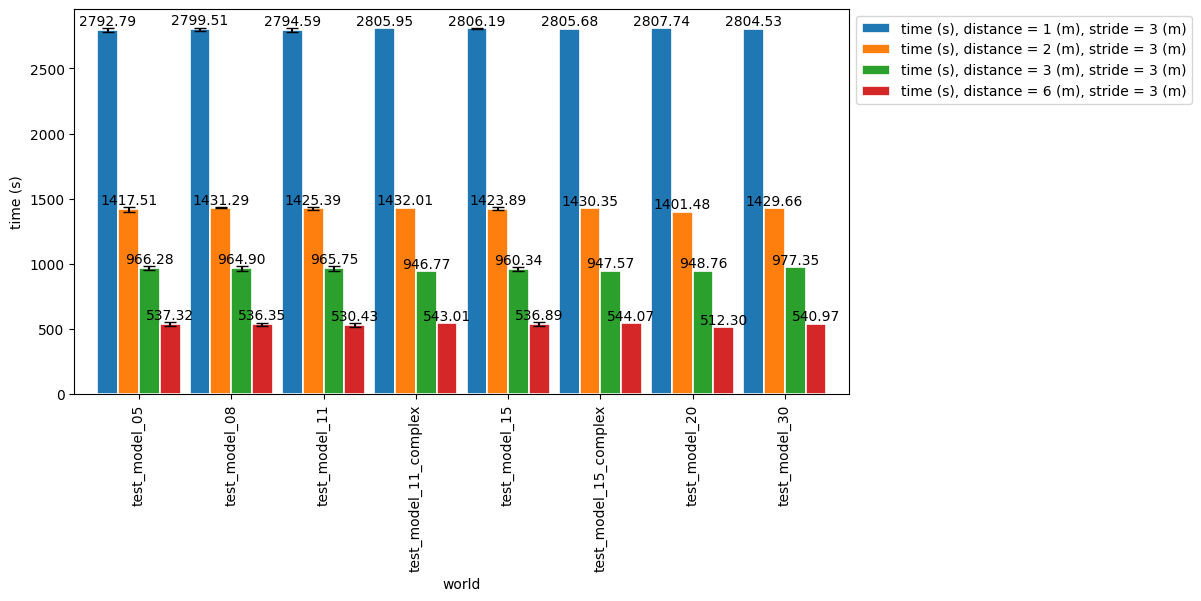
\includegraphics[width=\linewidth]{graphics/ski_nordique-time_vs_world_for_each_d.png}
		\caption{Runtime based on world density.}
		\label{fig:ski_nordique-time_vs_world_d}
	\end{subfigure}
	\caption{Evolution of Cohen's $\kappa$ and the execution time of the \textit{Nordic Skiing} algorithm as a function of the density of the world for different values of the distance between the two crawlers.}
	\label{fig:ski_nordique-world_d}
\end{figure}

We have very similar results to those obtained for the \textit{Roller Painting} algorithm.
Indeed, we observe in figure~\ref{fig:ski_nordique-kappa_vs_world_d} that the Cohen score generally decreases when the density of the world increases.
Moreover, the execution time of the algorithm \textit{Nordic Skiing}, observed in figure~\ref{fig:ski_nordique-time_vs_world_d}, is constant for each value of the density of the world.

\begin{figure}[h!]
	\centering
	\begin{subfigure}[t]{0.9\linewidth}
		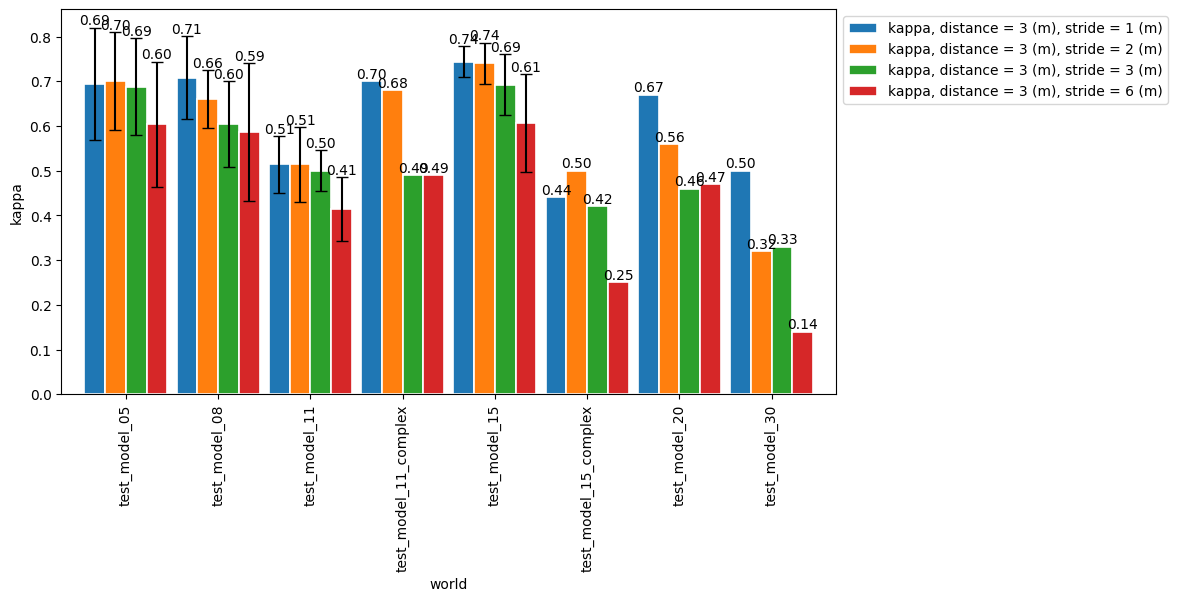
\includegraphics[width=\linewidth]{graphics/ski_nordique-kappa_vs_world_for_each_s.png}
		\caption{$\kappa$ according to the density of the world.}
		\label{fig:ski_nordique-kappa_vs_world_s}
	\end{subfigure}
	\hfill
	\begin{subfigure}[t]{0.9\linewidth}
		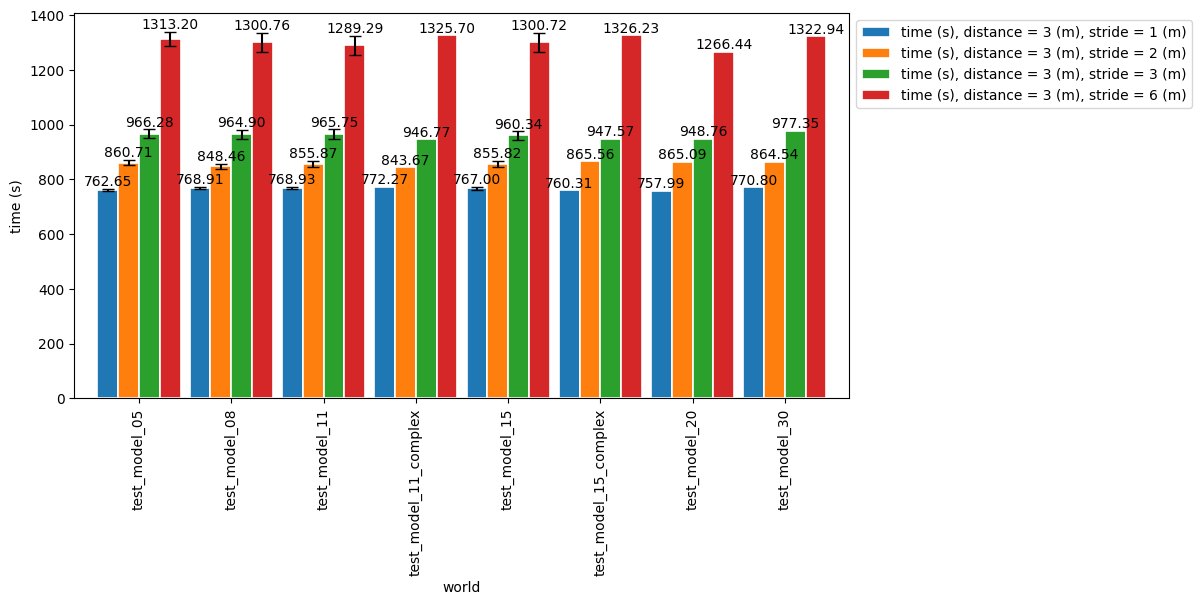
\includegraphics[width=\linewidth]{graphics/ski_nordique-time_vs_world_for_each_s.png}
		\caption{Runtime based on world density.}
		\label{fig:ski_nordique-time_vs_world_s}
	\end{subfigure}
	\caption{Evolution of Cohen's $\kappa$ and the execution time of the \textit{Nordic Skiing} algorithm according to the density of the world for different values of the stride between the two crawlers.}
	\label{fig:ski_nordique-world_s}
\end{figure}

We can observe in the figure~\ref{fig:ski_nordique-world_s} the evolution of the Cohen score and the execution time of the algorithm \textit{Nordic Skiing} according to the density of the world for different values of the stride $s$ between the two crawlers, and a distance $d = 3$ meters between the crawlers.
in the figure~\ref{fig:ski_nordique-kappa_vs_world_s}, we observe that the Cohen score is the lowest for large values of densities and large values of $d$, as for $d = 6$ meters and the maps with 30 and 20 corrosion areas.
This is explained by the fact that for large values of densities and $d$, the probability that the signal rays cross corrosion zones is higher.
There is therefore a greater chance that phantom zones will be created, which lowers Cohen's score.
The elongated shapes of the corrosion zones are also a factor that lowers the Cohen score as studied previously.
This is why we observe that the Cohen score is the highest for the map with the smallest density and without elongated forms of corrosion, that is to say the map with 15 corrosion zones.

In figure~\ref{fig:ski_nordique-time_vs_world_s}, we observe that the execution time of the algorithm \textit{Nordic Skiing} is constant for each value of the density of the world.
This was expected as for the \textit{Roller Painting} strategy.
However, we observe that the execution time varies with the stride $s$ used.
We would have rather expected the execution time to remain constant with the pitch of the crawlers.
Indeed, regardless of the value of the stride, the vertical and horizontal distance to be covered by the crawlers remains the same.
This significant difference in execution time is due to the way we implemented the \textit{Nordic Skiing} algorithm, which is not optimal.
We did not make the crawlers stop at the ends of the plates, but we made them continue by a value of the stride $s$, in addition, for simplicity of implementation, without thinking that the impact on the time of execution would be significant.

\begin{figure}[h!]
	\begin{subfigure}[t]{0.49\linewidth}
		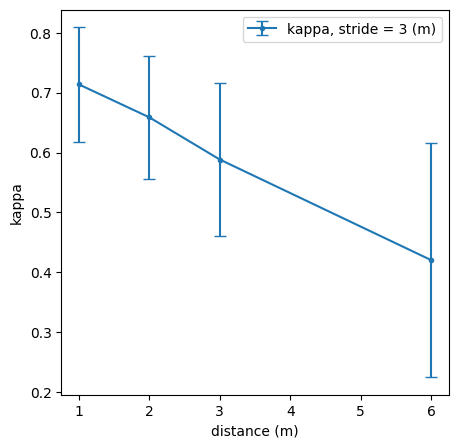
\includegraphics[width=\linewidth]{graphics/ski_nordique-kappa_vs_distance.png}
		\caption{$\kappa$ according to the distance between the two crawlers.}
		\label{fig:ski_nordique-kappa_vs_distance}
	\end{subfigure}
	\hfill
	\begin{subfigure}[t]{0.49\linewidth}
		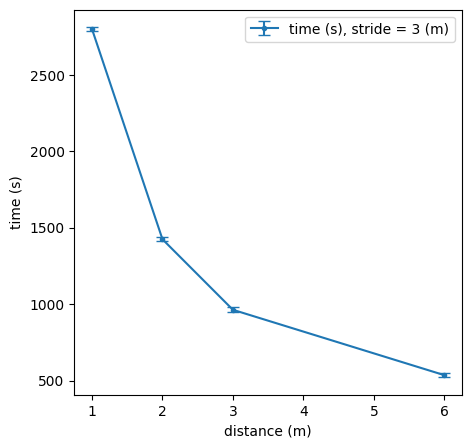
\includegraphics[width=\linewidth]{graphics/ski_nordique-time_vs_distance.png}
		\caption{Runtime according to the distance between the two crawlers.}
		\label{fig:ski_nordique-time_vs_distance}
	\end{subfigure}
	\caption{Evolution of Cohen's $\kappa$ and the execution time of the \textit{Nordic Skiing} algorithm according to the distance between the two crawlers.}
	\label{fig:ski_nordique-distance}
\end{figure}

In the figure~\ref{fig:ski_nordique-distance}, we observe the evolution of the Cohen score and the execution time of the algorithm \textit{Nordic Skiing} according to the distance which separates the two crawlers for a stride of 3 meters.
The score seems, as for the strategy \textit{Roller Painting}, to follow a linear relation with the distance which separates the two crawlers.
Execution time also appears to follow a linear relationship with the distance between the two crawlers.
The fact that the curve in figure~\ref{fig:ski_nordique-time_vs_distance} is not a straight line is due to the fact that the smaller the distance between the crawlers, the greater the number of rotations that the crawlers must perform.
However, the rotation time is not negligible in the execution times of the algorithms.

\begin{figure}[h!]
	\begin{subfigure}[t]{0.49\linewidth}
		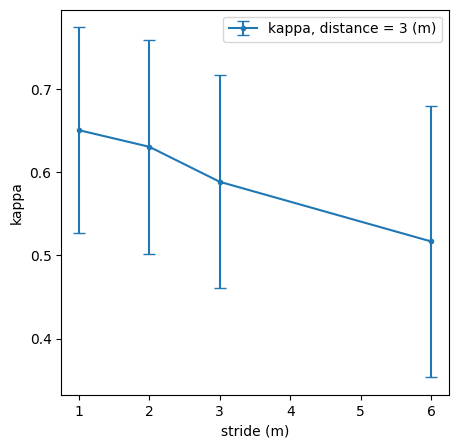
\includegraphics[width=\linewidth]{graphics/ski_nordique-kappa_vs_stride.png}
		\caption{$\kappa$ according to crawler stride.}
		\label{fig:ski_nordique-kappa_vs_stride}
	\end{subfigure}
	\hfill
	\begin{subfigure}[t]{0.49\linewidth}
		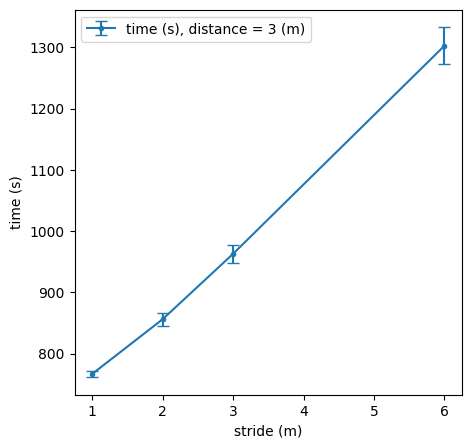
\includegraphics[width=\linewidth]{graphics/ski_nordique-time_vs_stride.png}
		\caption{Runtime according to crawler stride.}
		\label{fig:ski_nordique-time_vs_stride}
	\end{subfigure}
	\caption{Evolution of Cohen's $\kappa$ and the execution time of the \textit{Nordic Skiing} algorithm according to the crawler stride.}
	\label{fig:ski_nordique-stride}
\end{figure}

In the figure~\ref{fig:ski_nordique-stride}, we observe the evolution of the Cohen score and the execution time of the algorithm \textit{Nordic skiing} according to the crawlers' stride $s$ for a distance $d = 3$ meters.
The score seems to follow a linear relationship with the stride of the crawlers.
The smaller the stride, the higher the score.
This is consistent with what we explained previously.
The larger the stride, the greater the chance of creating phantom zones and therefore of reducing Cohen's score.
It should be noted however that there is a large variation in the score for the different values of the stride.
It therefore seems that the impact of the value of the stride on the score is rather weak unlike the impact of the value of the distance on the score.
Execution time seems to follow a linear relationship with crawler pace.
As explained previously, the latter should have been constant, but our implementation makes the execution time depend on the stride of the crawlers.

Again, it seems that the score and execution time are not affected by whether the shapes are complex or not.

In the rest of this report, we will consider a distance $d = 3$ between the two crawlers and a stride $s = 3$ for the algorithm \textit{Nordic Skiing}.

\subsection*{\textit{Polygonal Investigation} Navigation Strategy}

We then tested the \textit{Polygonal Investigation} algorithm on worlds composed of 5, 8 and 11 corrosion zones.
The inspection strategy is based on the results of the \textit{Roller Painting} strategy.
As explained previously, we justify this choice by the fact that the \textit{Roller Painting} strategy is the fastest of the \textit{a priori} strategies that we have implemented.

\begin{figure}[h!]
	\begin{subfigure}[t]{0.9\linewidth}
		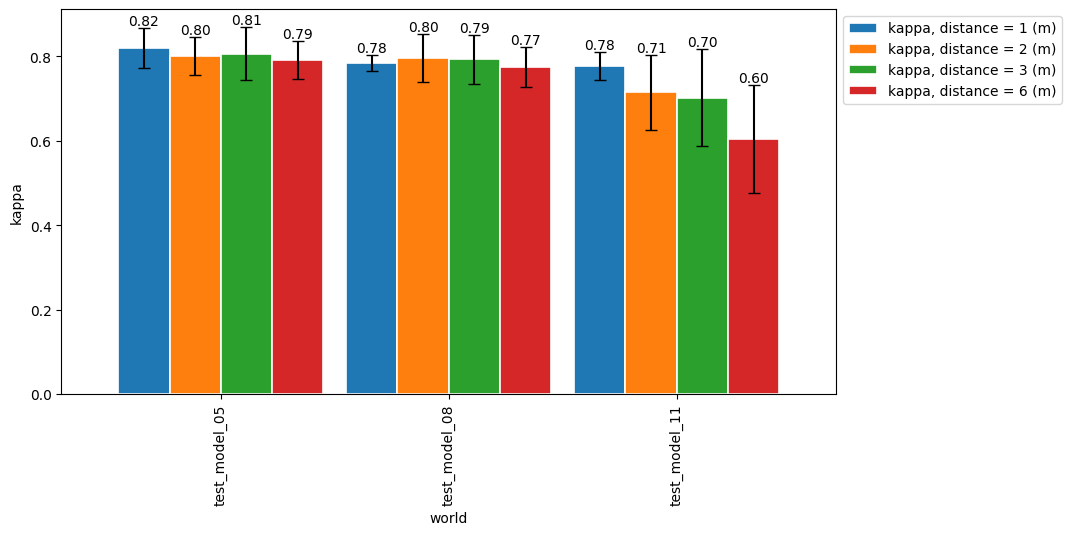
\includegraphics[width=\linewidth]{graphics/investigation_polygonale-kappa_vs_world_for_each_d_k1_n2_p4.png}
		\caption{$\kappa$ according to the density of the world.}
		\label{fig:investigation_polygonale-kappa_vs_world_for_each_d_k1_n2_p4}
	\end{subfigure}
	\hfill
	\begin{subfigure}[t]{0.9\linewidth}
		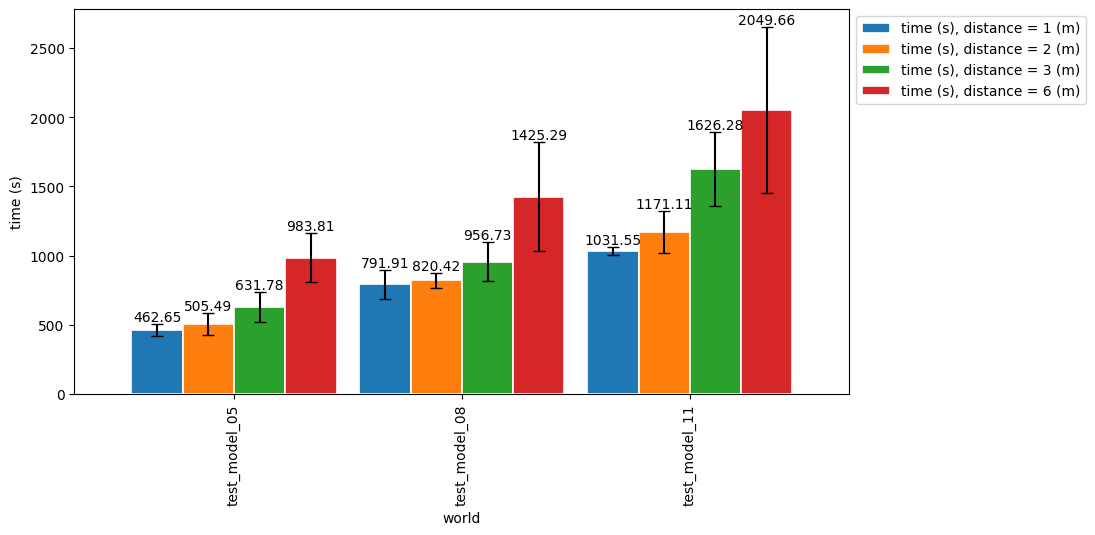
\includegraphics[width=\linewidth]{graphics/investigation_polygonale-time_vs_world_for_each_d_k1_n2_p4.png}
		\caption{Runtime based on world density.}
		\label{fig:investigation_polygonale-time_vs_world_for_each_d_k1_n2_p4}
	\end{subfigure}
	\caption{Evolution of Cohen's $\kappa$ and \textit{Polygonal Investigation} algorithm runtime according to the world density for different distances between crawlers with a 4-sided polygon.}
	\label{fig:investigation_polygonale-world_for_each_d_k1_n2_p4}
\end{figure}

The figure~\ref{fig:investigation_polygonale-kappa_vs_world_for_each_d_k1_n2_p4} shows the evolution of the Cohen score according to the density of the world for each value of $d$ used in the strategy \textit{Roller Painting}.
We used a 4-sided investigation polygon.
First, we observe Cohen scores relatively independent of distance between crawlers for maps with 5 and 8 corrosion zones.
This is an exciting result, because it means that we can use the \textit{Polygonal Investigation} strategy based on the results of the \textit{Roller Painting} strategy using a large distance between the crawlers, and therefore, a very fast \textit{Roller Painting} strategy.
Nevertheless, we can observe that for maps with 11 corrosion zones, the Cohen score is impacted by the distance between the crawlers, when the latter increases.
We attribute this result to the fact that this map has elongated corrosion zones very close to each other, having the effect of blocking certain rays emitted and received during the polygonal inspection of an area.
Polygonal inspection is therefore naturally impacted by the density of the world.
However, we can imagine, when repairing metal structures, that it is more convenient to merge corrosion areas close to each other into a single corrosion area, although this is not considered in our problem.

Figure~\ref{fig:investigation_polygonale-time_vs_world_for_each_d_k1_n2_p4} shows the evolution of execution time according to the world density for each value of $d$ used in the strategy \textit{Roller Painting}.
We used a 4-sided investigation polygon.
We observe that the execution time increases with the density of the world in a linear way.
This is an expected result, because the \textit{Polygonal Investigation} algorithm has linear complexity as a function of the number of corrosion zones, the latter consisting in traversing all the potential corrosion zones and inspecting them.
We also observe that the execution time increases with the distance between the crawlers.
Indeed, the greater the distance between the crawlers, the greater the number of phantom zones at the end of the \textit{Roller Painting} navigation strategy, and therefore the greater the number of potential corrosion zones.
However, these phantom areas are quickly processed by the \textit{Polygonal Investigation} algorithm.
For example, for map 5 with 11 corrosion areas, we get 12 potential corrosion areas with a distance of 1 meter between crawlers after the \textit{Roller Painting} strategy, versus 20 potential corrosion areas with a distance of 6 meters between the crawlers.
However, we observe an execution time of 1027 seconds for the first configuration versus 1616 seconds for the second configuration.
So we have for a 67\% increase in the number of potential corrosion areas, a 57\% increase in execution time.
The performance gain is not very large, but is still significant.

\begin{figure}[h!]
	\begin{subfigure}[t]{0.9\linewidth}
		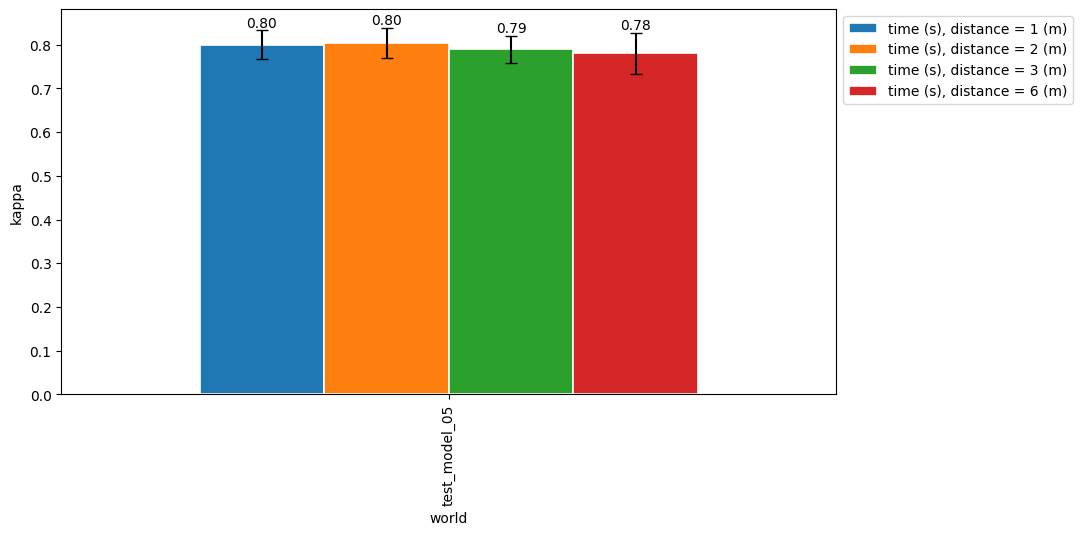
\includegraphics[width=\linewidth]{graphics/investigation_polygonale-kappa_vs_world_for_each_d_k1_n2_p6.png}
		\caption{$\kappa$ according to the density of the world.}
		\label{fig:investigation_polygonale-kappa_vs_world_for_each_d_k1_n2_p6}
	\end{subfigure}
	\hfill
	\begin{subfigure}[t]{0.9\linewidth}
			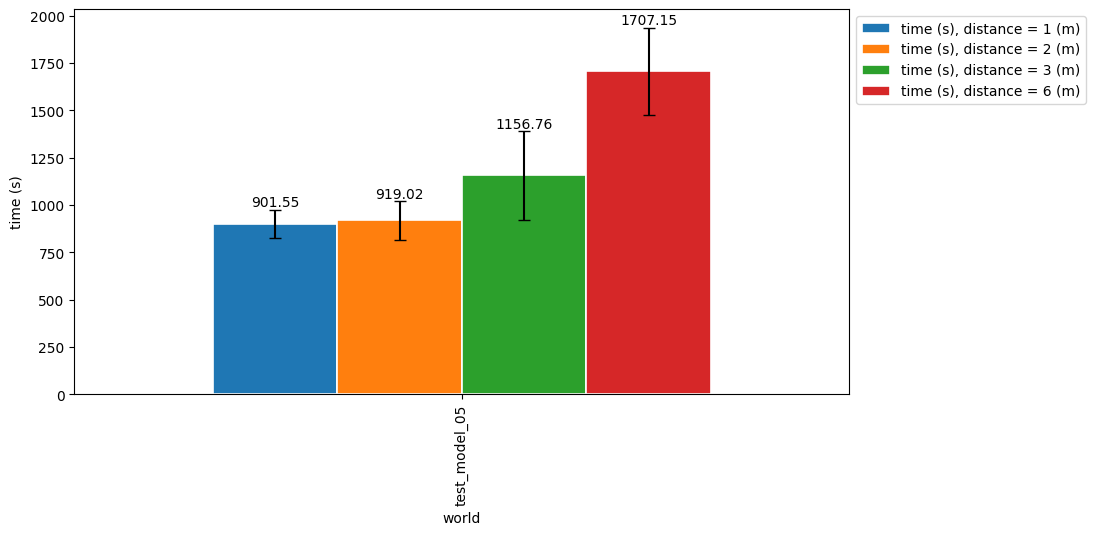
\includegraphics[width=\linewidth]{graphics/investigation_polygonale-time_vs_world_for_each_d_k1_n2_p6.png}
			\caption{Runtime based on world density.}
			\label{fig:investigation_polygonale-time_vs_world_for_each_d_k1_n2_p6}
	\end{subfigure}
	\caption{Evolution of Cohen's $\kappa$ and \textit{Polygonal Investigation} algorithm runtime according to the world density for different distances between crawlers with a 6-sided polygon.}
	\label{fig:investigation_polygonale-world_for_each_d_k1_n2_p6}
\end{figure}

We also varied the size of the investigation polygon of the \textit{Polygon Investigation} strategy.
We present in figure~\ref{fig:investigation_polygonale-kappa_vs_world_for_each_d_k1_n2_p6} the evolution of the Cohen score as a function of the density of the world for map 5, for a polygon with 6 vertices.
First, we do not observe a significant improvement in the Cohen score when the size of the investigation polygon increases.
On the contrary, we observe an average decrease, although very weak, of the score.
In theory, increasing the size of the investigation polygon should make it possible to better approach the convex hull of the corrosion zones, and therefore to obtain a better Cohen score.
However, we are limited in our implementation by the resolution used for the discretization of the map.
% Thus, it is probable that increasing the size of the investigation polygon eliminates cells from the occupancy grid (at the periphery of the corrosion zones) where corrosion is actually present, because it has there existed a ray which crossed this same cell.
However, for a more precise resolution, we should observe an improvement in the Cohen score.

We present in the figure~\ref{fig:investigation_polygonale-time_vs_world_for_each_d_k1_n2_p6} the evolution of the execution time according to the density of the world for map 5, for a polygon with 6 vertices.
Here, we naturally observe an increase in execution time when the size of the investigation polygon increases.

We would also have liked to vary the number of robots used for the polygonal investigation as well as the number of robot teams.
However, we did not have time to implement a solution for managing collisions between robots.
It would be interesting in future work to implement such a solution and to analyze the performance of the \textit{Polygonal Investigation} algorithm with these different parameters.
Indeed, the execution time of the \textit{Polygonal Investigation} algorithm should decrease when $k$ and $n$ increase.

In the next subsection, we will compare the performance of the \textit{Polygonal Investigation} algorithm with those of the \textit{Roller Painting} and \textit{Nordic Skiing} algorithms.
To do this, we will consider an investigation polygon, for the polygonal investigation, with $p = 4$ vertices.

